\documentclass[dvipdfmx]{jsarticle}
\usepackage[dvipdfmx]{graphicx}
\usepackage{amsmath, amssymb}
\usepackage{mathtools}
\usepackage{here}
\usepackage{url}
\begin{document}
\title{週間進捗報告}
\author{権藤陸}
\date{2022年6月1日}
\maketitle
\section{進捗}
"Person Reidentification Based on Automotive Radar Point Clouds"を読み始めた.
\section{本研究の概要}
人物のRe-identification(ReID)を,現在主流のLiDARやカメラを用いて行うのではなく,低コスト(LiDARと比較して1/100以下)な車載レーダを用いて行うことを試みる.

\begin{figure}[htbp]
\begin{center}
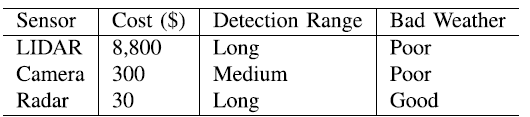
\includegraphics[width=0.6\linewidth]{./comparison_of_sensors.png}
\end{center}
\caption{センサの比較}
\end{figure}

本研究は,4次元レーダ点群から時空間情報を抽出するための深層学習ネットワークを設計する.
データセットは,本研究のために収集されたもので,15人分の通常データセットと40人分の認識が困難なデータセットを用意した.
評価結果から,我々の手法はReIDタスクにおいて91\%のCMC-1精度を達成することが分かった.また,人物再識別タスクにおいても,15人および40人に対して,それぞれ98\%および91\%の精度を達成した
実験の結果,レーダーを用いたReIDはプライバシーを守るだけでなく,低照度環境や衣服が大幅に変化する場合に,カメラベースのReIDを上回る性能を示すことが分かった.

\newpage

\section{車載レーダ}
車載レーダについてのイメージを明確にするため,簡単に車載レーダについて調べた.本研究で用いられたレーダは,Texas Instruments社の 77GHz FMCWレーダのAWR1843というモデルである.

\begin{figure}[H]
\begin{center}
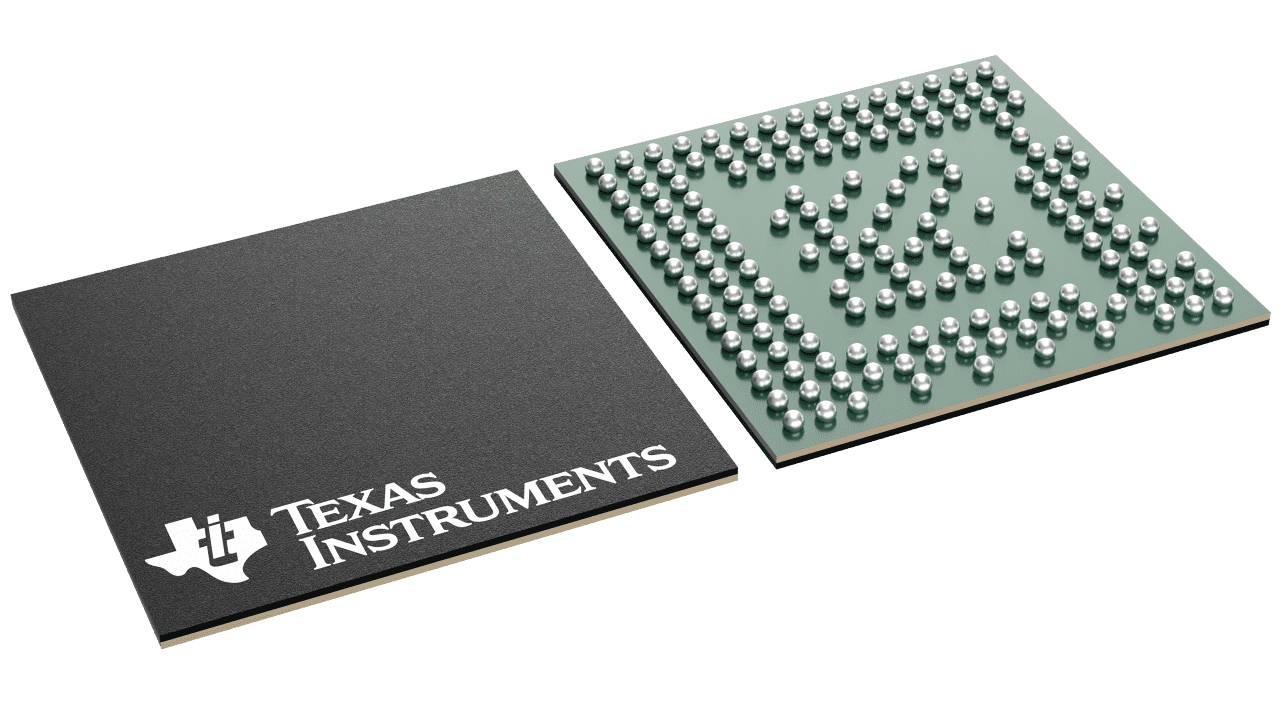
\includegraphics[width=0.5\linewidth]{./abl0161b.png}
\end{center}
\caption{本研究で用いられた車載レーダ:AWR1843}
\end{figure}

下図のように,前方に向けてレーダでミリ波を生成,送信し,前方の車に反射した信号を受信アンテナで受け取り,対象物との距離を測る.短波長のミリ波のため,最小 0.1 mm 単位の動きを検出可能である.
\begin{figure}[H]
\begin{center}
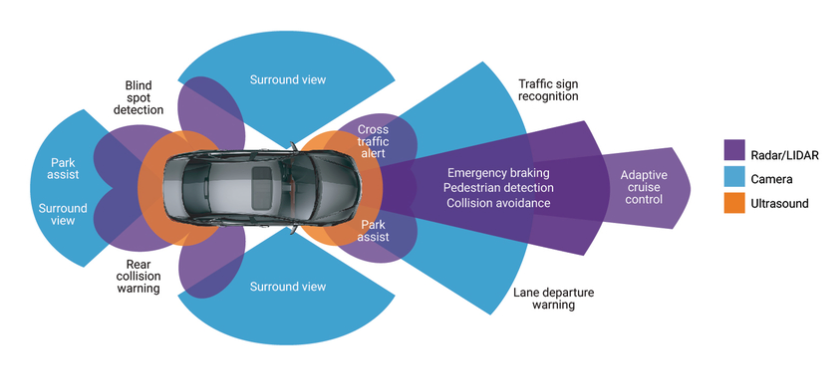
\includegraphics[width=0.8\linewidth]{./adas_system.png}
\end{center}
\caption{Advanced Driver Assistance Systems}
\end{figure}

\section{導入}
現在,社会的に広く人物認証システムが用いられており,その多くは顔認証によって行われている.
しかし,顔認証は難しく,人物が非協力的であったり,障害物,視点が異なる場合等は失敗することが多い.
そこで,ReIDが注目を集めている.現在のReIDはカメラベースで,人物の服の色や髪型など,外見から得られる情報を用いているため,照度や背景などの環境変化に弱い.
また,カメラベースのため,プライバシーの問題も発生する.
今回用いるレーダは77GHzのミリ波を発し,人体のエコー信号を取得することで,距離,方向,瞬間速度を測定可能である.
特長として,環境変化に強くロバストであり,服の色などから影響を受けず,最終的に生成されるのは点群であるため,
認識対象人物のプライバシーも守られる.

本論文の主な貢献は以下の3つである.
\begin{itemize}
	\item 著者らの知る限り,実世界のシーンにおける人物ReID問題で市販の自動車レーダーの点群を用いたのは著者らが初めてである.
	\item ドップラー速度情報を追加で含む4次元レーダー点群から直接特徴を学習できる新しい深層学習アーキテクチャと,Bi-LSTMを用いてマルチフレームレーダーデータの変化するスパース点群から時空間情報を抽出すること.
	\item 人物ReID問題へのレーダー適用の可能性を示すデモと,実際のレーダーデータを用いた評価について直感的な説明と分析を行うことができる.
\end{itemize}
\section{計画}
引き続き論文を読み進める.
\begin{itemize}
	\item FMCWレーダの原理の理解
    \item 提案されたモデルの理解
\end{itemize}
\end{document}